\documentclass[tikz]{standalone}

\usepackage[greek,english]{babel}

\usepackage{pgfplots}
\usetikzlibrary{decorations.pathreplacing}

\pagecolor{white}

\begin{document}
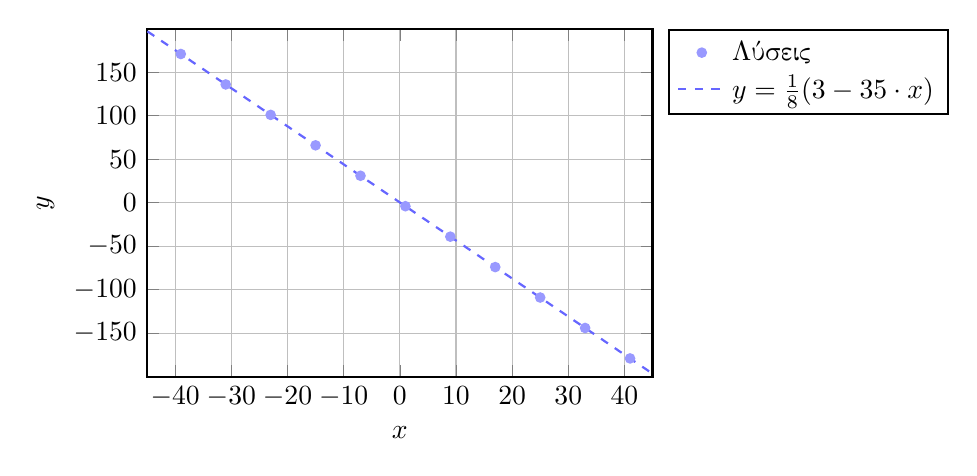
\begin{tikzpicture}
\begin{axis}[
    width=8cm,
    height=6cm,
    domain=-15:15, 
    xmin=-45,
    xmax=45,
    ymin=-200,
    ymax=200,
    thick,
    ytick={-150,-100,-50,0,50,100,150},
    xtick={-40,-30,-20,-10,0,10,20,30,40},
    legend pos=outer north east,
    mark size=1.5pt,
    xlabel={$x$},
    ylabel={$y$},
    legend cell align={left},
    grid]


\addplot[only marks, blue!40!white] coordinates {
(-47, 206)
(-39, 171)
(-31, 136)
(-23, 101)
(-15, 66)
(-7, 31)
(1, -4)
(9, -39)
(17, -74)
(25, -109)
(33, -144)
(41, -179)
(49, -214)
};
\addlegendentry{\textgreek{Λύσεις} }

\addplot[red, domain=-50:50,restrict y to domain=-200:200, samples=100, blue!60!white,dashed]  {(3 - 35 * x) / 8 };

\addlegendentry{$y = \frac{1}{8} (3 - 35 \cdot x)$ }

\end{axis}
\end{tikzpicture}
\end{document}
